\section{Алгоритм построения изображения}

К алгоритму построения алгоритма приведены следующие требования:
\begin{itemize}
    \item на вход подаётся список объектов сцены, описание источника света и камеры;
    \item на выход подаётся построенное изображение.
\end{itemize}

Алгоритм построения изображения представлен на рисунке~\ref{fig:rendering}.

\begin{figure}[h!]
    \centering
    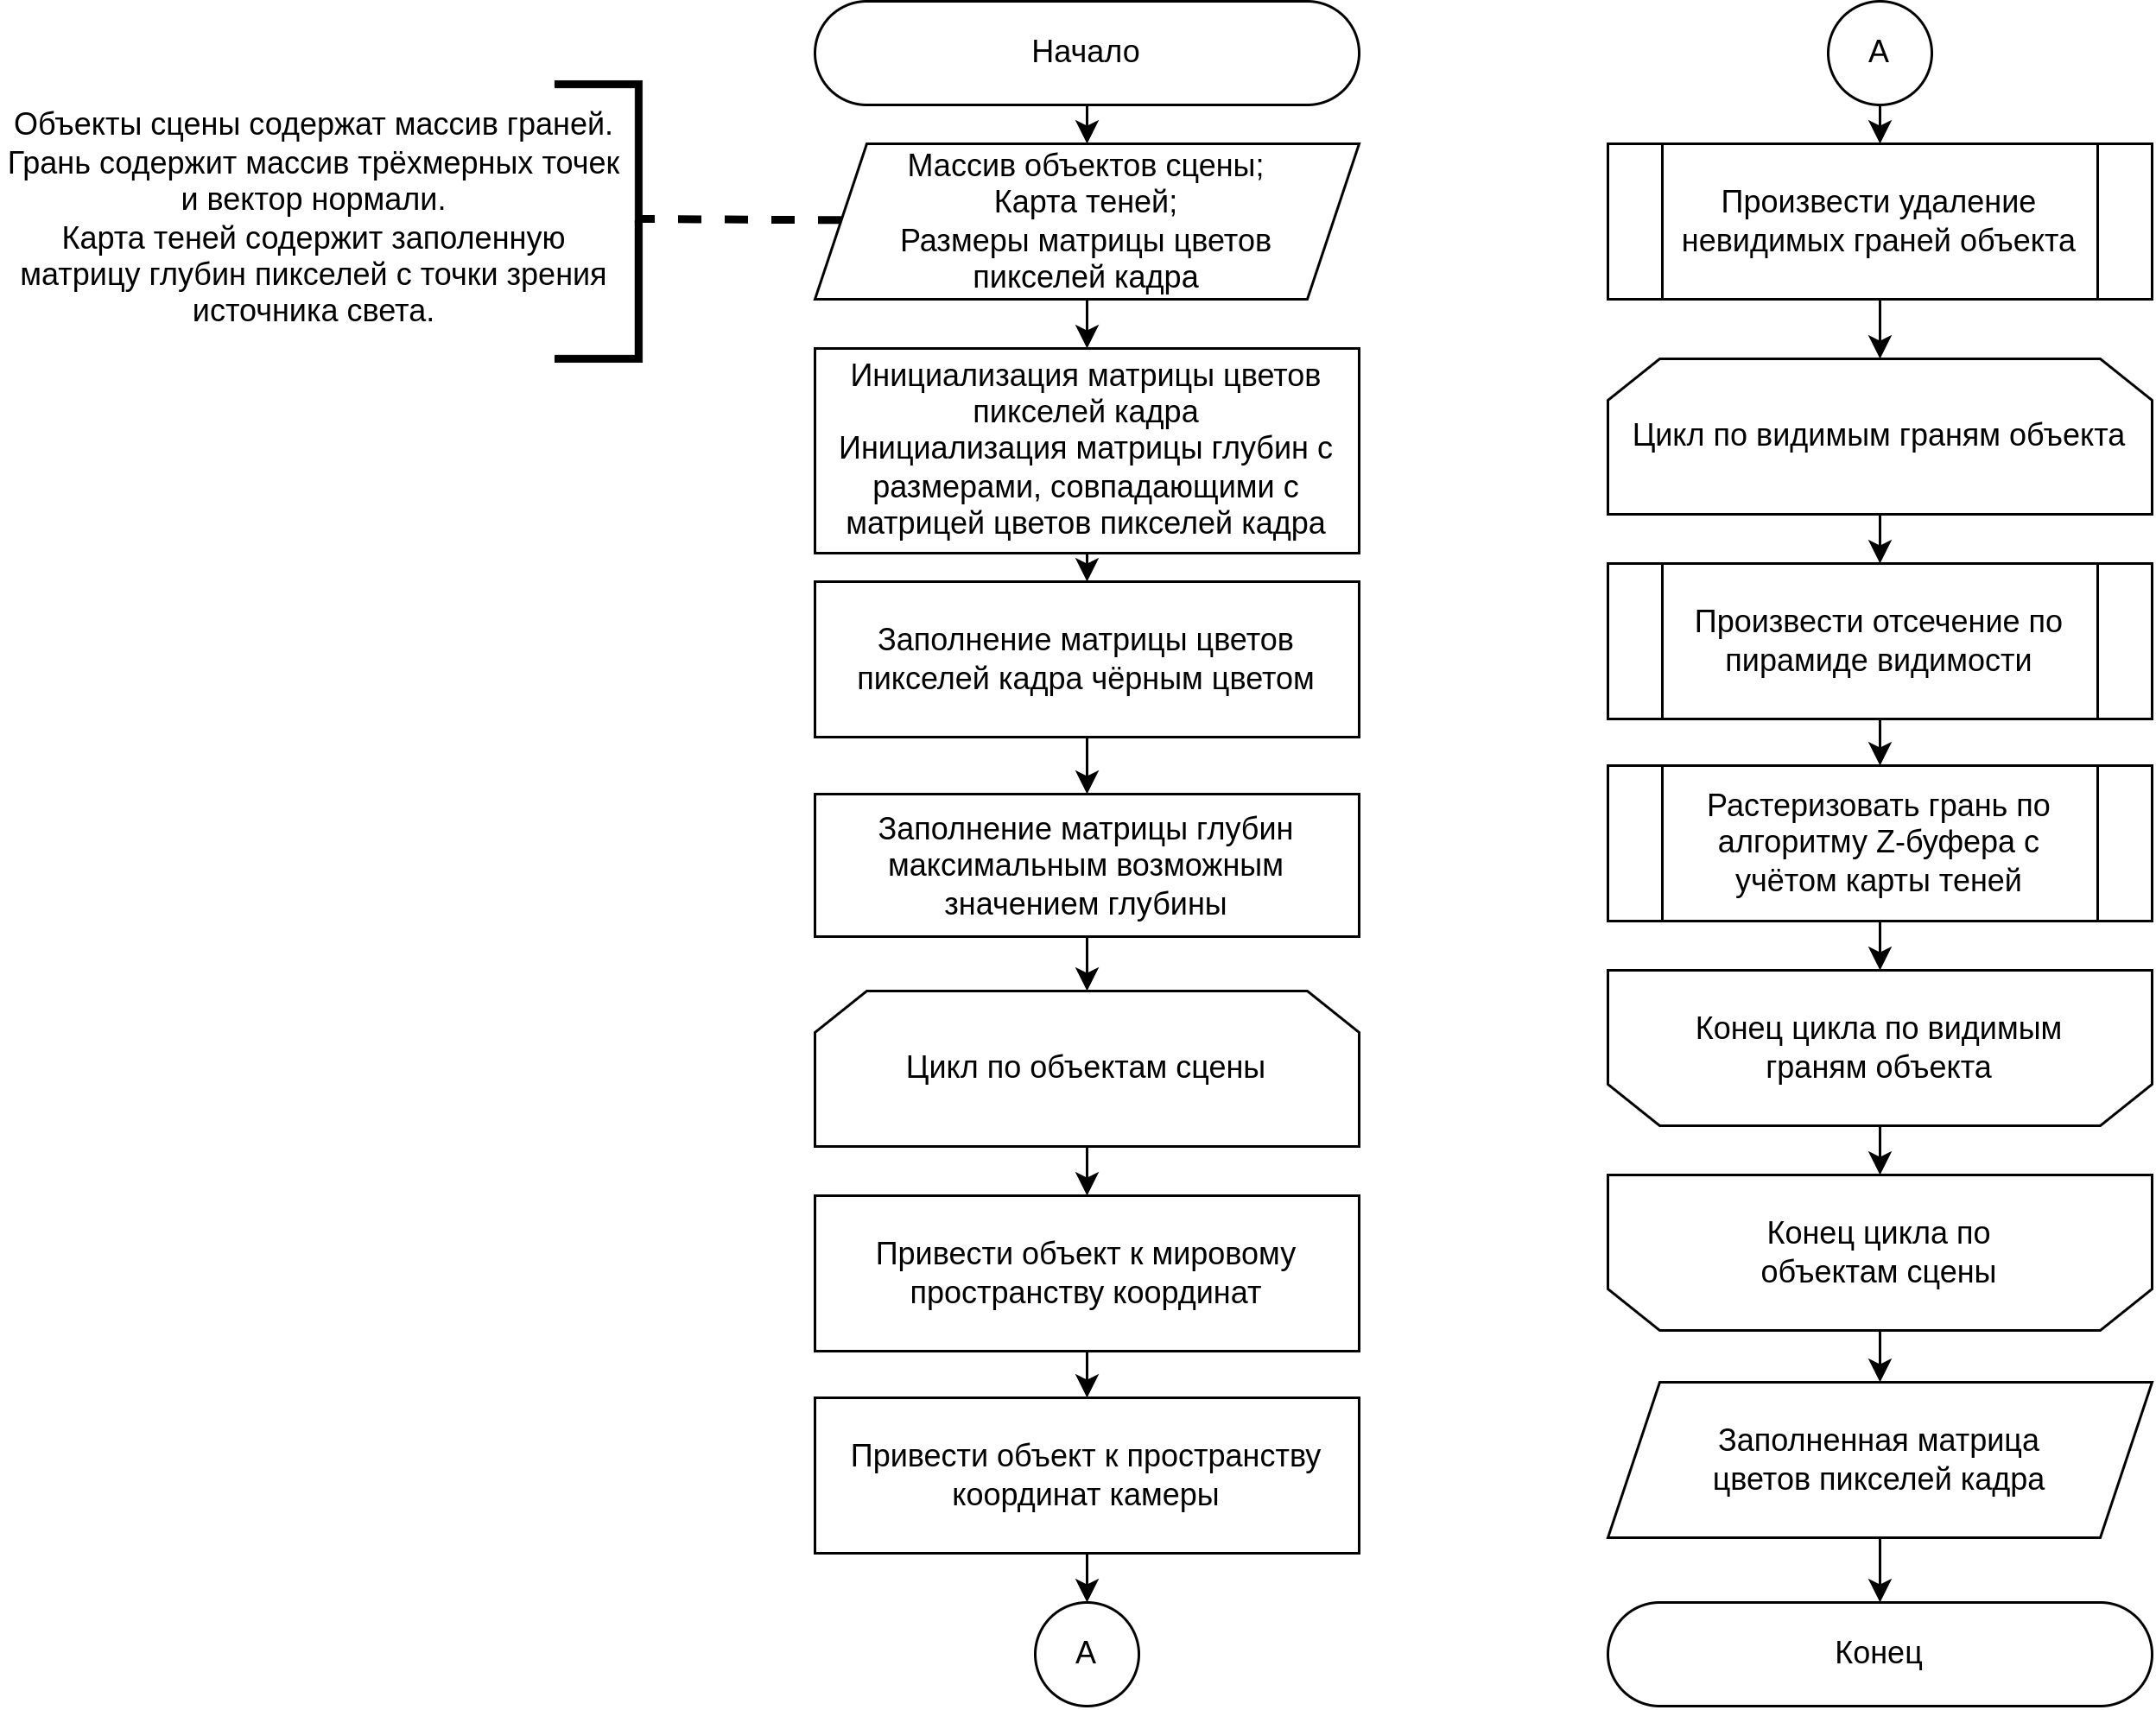
\includegraphics[width=.5\textwidth]{rendering.drawio.png}
    \caption{Алгоритм построения изображения}
    \label{fig:rendering}
\end{figure}

В следующих пунктах будут подробнее описаны этапы данного алгоритма.